\chapter*{TD3 :  Fonction d'une variable aléatoire : exemples concrets.}

\setcounter{exercice}{0}

\begin{mdframed}
\begin{exercice}
Dans cet exercice, lorsqu'est demandé de préciser la loi d'une variable aléatoire, on donnera la fonction de répartition, et si cela a un sens, la densité.

\begin{enumerate}
    \item On suppose que $X$ suit la loi uniforme sur $[0, 1]$, notée $\mathcal{U}(0, 1)$. Quelle loi suit $X^2$ ?
    \item On suppose que $X^2$ suit la loi uniforme sur $[0, 1]$, et $\mathbb{P}(X \geq 0) = 1$. Quelle loi suit $X$ ?
    \item On suppose que $X$ suit la loi uniforme sur $[0, \pi]$. Quelle loi suit $\cos(X)$ ?
    \item On suppose que $\cos(X)$ suit la loi uniforme sur $[-1, 1]$, et $\mathbb{P}(X \in [0, \pi]) = 1$. Quelle loi suit $X$ ?
\end{enumerate}
\end{exercice}
\end{mdframed}

\medskip

\begin{mdframed}
\begin{exercice}
Soit $X$ une variable aléatoire de loi $\mathcal{E}(\alpha)$, pour $\alpha > 0$.

\begin{enumerate}
    \item Quelle loi suit $\alpha X$ ?
    \item Quelle loi suit $Y = e^X$ ?
\end{enumerate}

On précisera dans les deux cas la valeur de la densité si la variable en admet une.
\end{exercice}
\end{mdframed}

\medskip

\begin{mdframed}
\begin{exercice}
Soit $X$ une variable aléatoire de loi $\mathcal{N}(0, 1)$.

\begin{enumerate}
    \item Quelle loi suit $\mu + \sigma X$, pour $\mu \in \mathbb{R}$, et $\sigma > 0$ ?
    \item Quelle loi suit $Y = X^2$. Reconnaître une loi $\Gamma(\alpha, \beta)$ pour des paramètres à préciser.
\end{enumerate}
\end{exercice}
\end{mdframed}

\medskip

\begin{mdframed}
\begin{exercice}
Un bout de bois est cassé en un point uniforme, formant deux bouts ; si l'on assimile le bout de bois à l'intervalle unité $[0, 1]$, quelle est la loi de la longueur du bout contenant la marque d'abscisse $p$, pour $p \in [0, 1]$ ? Quelle loi retrouve-t-on lorsque $p = 1/2$ ?
\end{exercice}
\end{mdframed}

\medskip

\begin{mdframed}
\begin{exercice}
Soit $X$ une variable aléatoire de loi $\mathcal{C}(a)$ pour $a > 0$, qui est la loi de densité $x \mapsto \frac{a}{\pi} \frac{1}{a^2 + x^2}$ sur $\mathbb{R}$.

\begin{enumerate}
    \item Calculer la fonction de répartition et en déduire que la fonction proposée est bien une densité.
    \item Quelle loi suit $X/a$ ?
    \item Quelle loi suit $Y = 1/X$ ?
\end{enumerate}

Pour la dernière question, on pourra librement utiliser la relation : pour $x \neq 0$, $\arctan(x) + \arctan(1/x) = \frac{\pi}{2} (\mathbb{1}_{\{x>0\}} - \mathbb{1}_{\{x<0\}})$.
\end{exercice}
\end{mdframed}

\medskip

\begin{mdframed}
\begin{exercice}
On considère un repère cartésien d'origine $O$ et $A$ le point de coordonnées $(0, -1)$. Pour $\Theta \in ]-\pi/2, \pi/2[$, il existe un unique point $B$ d'ordonnée $-1$ que l'angle $\widehat{AOB}$ est de $\Theta$ radians ; on note alors $X$ l'abscisse de $B$.

Ci-dessous, deux valeurs d'angles possibles : $\Theta > 0$ et $\Theta' < 0$, et les points $B$ et $B'$ correspondants :

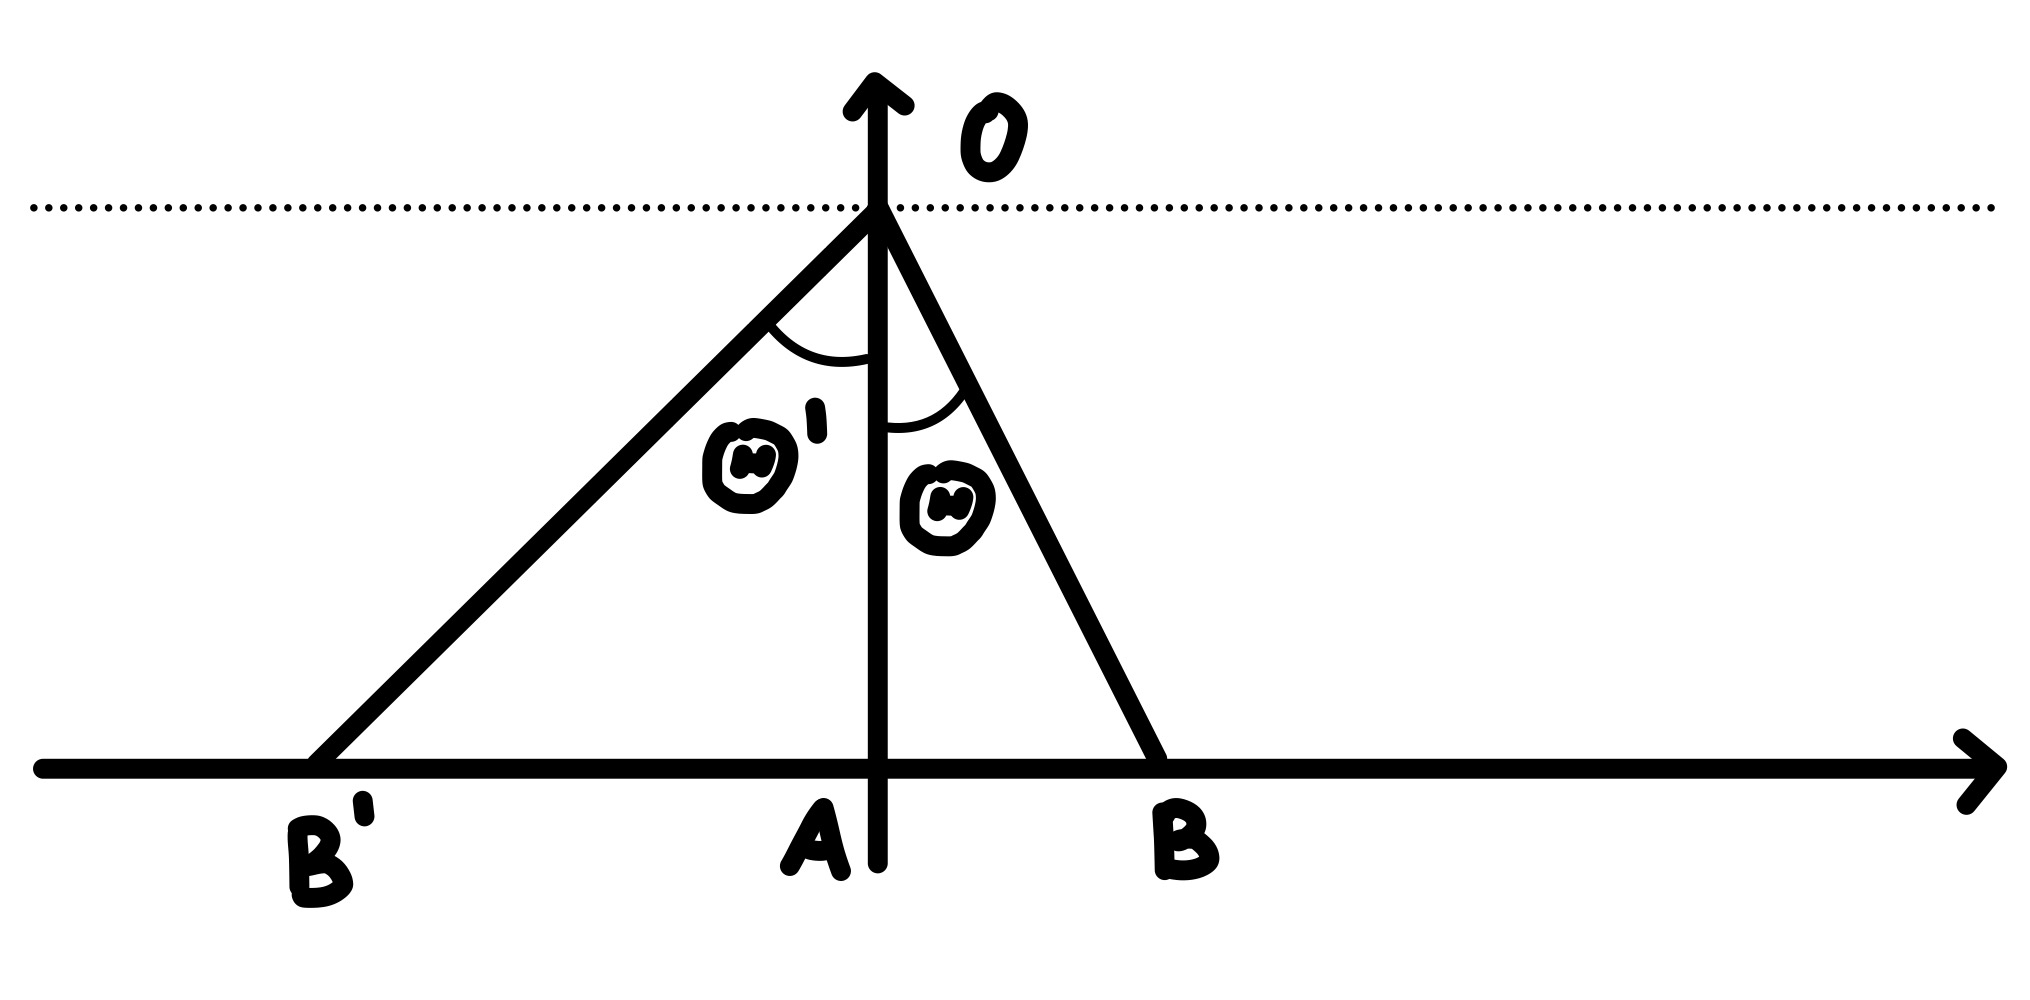
\includegraphics[width=10cm]{Cours1/Im.jpg}

Si $\Theta$ suit la loi uniforme sur $]-\pi/2, \pi/2[$, montrer que $X$ suit la loi $\mathcal{C}(1)$.
\end{exercice}
\end{mdframed}

\medskip

\begin{mdframed}
\begin{exercice}[Simulation à partir de la loi uniforme.] 
Soit $F$ fonction de répartition qui réalise une bijection d'un intervalle $I$ sur $]0, 1[$, et $U$ une variable aléatoire de loi $\mathcal{U}(0, 1)$.

\begin{enumerate}
    \item Quelle est la fonction de répartition de $F^{-1}(U)$ ? En déduire la loi de $F^{-1}(U)$.
\end{enumerate}
Préciser $I$ pour les deux lois suivantes, la bijection réciproque $F^{-1} : ]0, 1[ \to I$ :
\begin{enumerate}
    \setcounter{enumi}{1}
    \item $F$ fonction de répartition de $\mathcal{E}(\lambda)$ pour $\lambda > 0$.
    \item $F$ fonction de répartition de $\mathcal{C}(a)$ pour $a > 0$.
\end{enumerate}
Application : Quelle est la loi de
\begin{enumerate}
    \setcounter{enumi}{3}
    \item $Z = -\frac{\ln U}{\lambda}$
    \item $W = a \tan\left(\pi\left(U - \frac{1}{2}\right)\right)$.
\end{enumerate}
\end{exercice}
\end{mdframed}

